\documentclass[12pt, a4paper]{article}

\usepackage[utf8]{inputenc}
\usepackage[russian]{babel}
\parindent 0pt
\parskip 8pt
\usepackage{amsmath}
\usepackage{amssymb}
\usepackage{array}
\usepackage[left=2.3cm, right=2.3cm, top=2.7cm, bottom=2.7cm, bindingoffset=0cm]{geometry} % headheight=0pt,
\usepackage{hyperref}
\usepackage{graphicx}
\usepackage{multicol}
\usepackage{fancyhdr} 
\usepackage{extramarks}
\usepackage[usenames,dvipsnames]{color}
\usepackage{titlesec}
\usepackage[normalem]{ulem}
\usepackage{tikz}
\definecolor{grey}{RGB}{128,128,128}

\pagestyle{fancy}
\fancyhf{}
\lhead{Билет № 1.4}
\chead{Кэш-память}
\rhead{\thepage}
\lfoot{made with Ы}
\cfoot{}
\rfoot{\today}
\renewcommand\headrulewidth{0.4pt}
\renewcommand\footrulewidth{0.4pt}

\titlespacing*{\section}{0pt}{5pt}{0pt}
\titlespacing*{\subsection}{0pt}{5pt}{0pt}
\titlespacing*{\subsubsection}{0pt}{5pt}{0pt}

\begin{document}
\textbf{Кэш} - небольшая быстрая память, расположенная близко к процессору (обычно на одном с ним кристалле). Обычно SRAM.
\section{Зачем?}
Потому что доступ к памяти долгий, а часто имеющиеся данные хотелось бы получать за быстро.
\section{Уровни кэша}
В современных архитектурах кэш делится на уровни, обычно на 3.
\begin{itemize}
    \item \textbf{L1} - кэш первого уровня. Содержит то, что активно используется, но не уместилось в регистры. Обычно делится на кэш для данных \textbf{L1d} и кэш для инструкций \textbf{L1i}. Обычный объём ~ 32КБ. Время доступа ~ 4 такта.
    \item \textbf{L2} - кэш второго уровня. Обычно общий для данных и для инструкций. Содержит часто используемые данные. Обычный объём ~ 256КБ. Время доступа ~ 12 тактов.
    \item \textbf{L3} - кэш третьего уровня. Содержит то, что еще успели закэшировать. Обычный объём ~ 8МБ. Время доступа ~ 50 тактов. Обычно общий для всех ядер.
    \begin{figure}[ht]
        \centering
        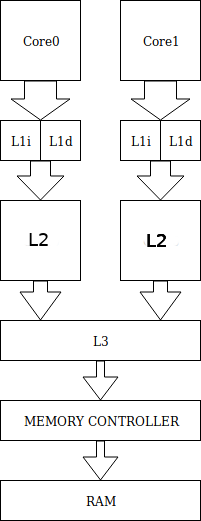
\includegraphics[scale=0.4]{./images/CACHElevels}
        \caption{Примерная схема. Чем ниже, тем тоньше шина}
        \label{fig:CACHElevels}
    \end{figure}
    Иногда встречается L4 кэш, но он обычно DRAM и находится вне CPU.
\end{itemize}
\section{Replacement police}
Чтобы записать куда-то новую кэш-линию при кэш-промахе, кэш должен освободить место. Существует несколько вариантов:\\
\begin{itemize}
    \item \textbf{LRU} (Least-recently used) - выкинуть самую давно использовавшуюся линию.
    \item \textbf{FIFO} {First In First Out} - выкинуть самую давно прочитанную в кэш линию.
\end{itemize}
\section{Политика чтения}
\subsection{Look-aside}
CPU отправляет запрос на чтение в память. Кэш подсматривает. Если не может ответить на запрос - не отвечает, если может - отвечает, а в память посылает отмену.\\
\begin{figure}[h]
    \centering
    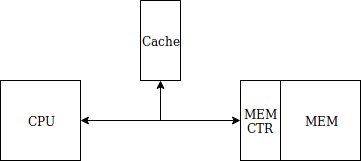
\includegraphics[scale=0.5]{images/LookAside.png}
    \caption{Look-aside}
    \label{fig:LookAside}
\end{figure}
Данные, которые еще не закэшированны читаются быстрее. 
\subsection{Look-through}
CPU отправляет запрос на чтение в кэш. Если у кэша есть нужная линия, он отвечает. Если нет, то запрашивает линию у основной памяти, а её ответ сохраняет себе.
\begin{figure}[h]
    \centering
    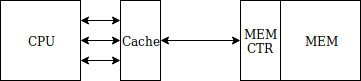
\includegraphics[scale=0.5]{images/LookThrough.png}
    \caption{Look-through}
    \label{fig:LookThrough}
\end{figure}
Если у нас кэш умный, у нас cache-hit в ~90\% запросов. А значит скорость обращения к памяти нам не очень важна, а вот скорость обращения к кэшу - очень. При look-through можем сделать \textbf{жирную} шину до процессора (т.к. они с кэшем на одном кристалле) и выиграть в скорости. А при look-aside - нет.
\section{Write policies}
\subsection{При cache-hit}
\subsubsection{Write-through}
Пишем и в кэш, и в память. Проще реализовать, но очередь к памяти забивается не очень полезными запросами (на запись в одну и ту же ячейку, например).
\subsubsection{Write-back}
Пишем только в кэш, когда линия вытесняется - записываем в память. Реализовать сложнее, т.к. нужно как-то запоминать, являются ли данные копией памяти (clean) или изменены (dirty). Эта штука быстрее, потому что в очереди к памяти не стоят бесполезные последовательные запросы на запись вида: записать в ячейку Х значение 1, записать в ячейку Х значение 2 и т.д.
\subsection{При cache-miss}
\subsubsection{Write allocate или fetch on write}
При кэш-промахе нужная кэш-линия сначала загружается в кэш, а потом в неё происходит запись. В таком случае промахи при записи аналогичны промахам при чтении.
\subsubsection{No-write allocate или write around}
При кэш-промахе пишем сразу в память, не подгружая ничего в кэш.
\subsection{Ещё про кэш}
Кэш - это быстрая SRAM память, а она занимает много места.\\ 
\begin{figure}[h]
    \centering
    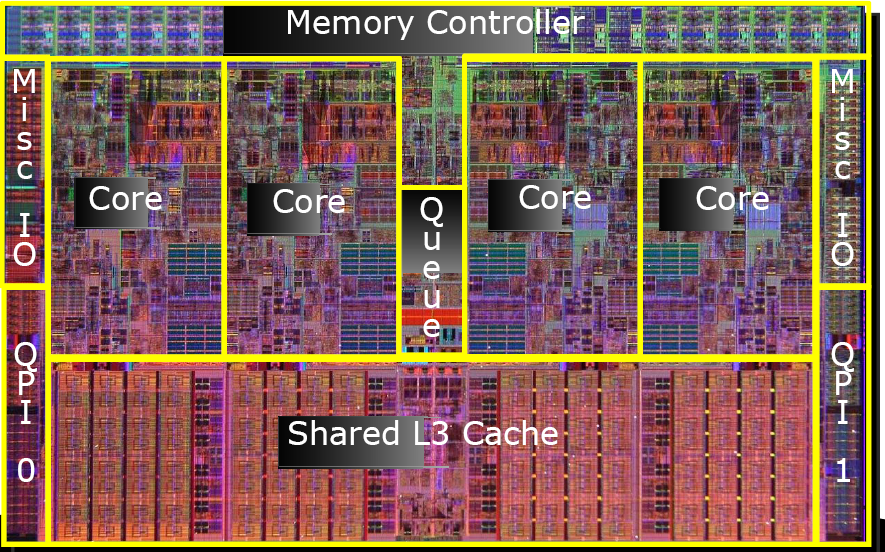
\includegraphics[width=0.6\linewidth]{./images/Core.png}
    \caption{Core i7}
    \label{fig:Core}
\end{figure}
Кроме того, ближе к реальности схема, когда у нас L3-кэш - это несколько маленьких кэшей, сидящих на одной шине, а не один большой. Таким образом повышается маштабируемость: у нас есть блок из CPU-L1-L2-L3, который можно размножать копипастой.
\section{Кэширование данных}
Если бы кэш кэшировал побайтово, то вместе с каждыми 8 битами данных мы хранили бы еще 32 бита адреса. Не очень выгодно, особенно учитывая что кэш - дорогое удовольствие (занимает до четверти кристалла, ы).\\
Данные кэшируются кэш-линиями. Обычно одна кэш-линия - 64 байта. Соотвественно адрес можно хранить один на кэш-линию. Кэш-линии не пересекаются! Т.е адрес кэш-линии должен быть кратен 64. Следовательно можем не хранить для линии младшие 6 бит адреса - это всё равно нули.
\begin{figure}[h]
    \centering
    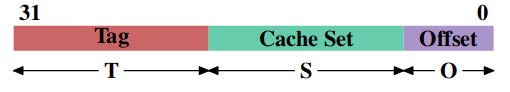
\includegraphics[width=0.6\linewidth]{./images/lineADDR.png}
    \caption{Как-то так разделяется адрес. Offset - адрес данных внутри кэш-линии}
    \label{fig:lineADDR}
\end{figure}
\section{Политика кэширования}
Поиск кэш-линии ведется по тэгу (блок T в адресе). Существует несколько способов организовать адрес.
\subsection{Полная ассоциативность}
Можем любой блок данных положить в любую строку кэша. Т.е. размер блока S в адресе равен 0.\\
Это значит, что нам нужно провести $2^T$ сравнений, где $T$ - размер тэга. Это очень много. Мы не можем делать сравнения последовательно (это долго, следовательно теряется весь смысл кэша), значит нам нужно $2^T$ аппаратных компараторов. Что-то многовато.
\subsection{Direct-mapping}
Другая крайность: пусть теперь размер тэга равен нулю.\\ Встречаем другую проблему: если мы обращаемся к блокам памяти, которые попадают в одну кэш-линию, то работа с ними получается даже немного медленнее, чем без кэша: мы постоянно вытесняем одни данные другими.
\subsection{Групповая ассоциативность}
Разделим кэш на $N$ групп по $M$ кэш-линий в каждой.\\
Пусть поступил запрос с адресом ячейки X. Последние $O$ ячеек - адрес внутри кэш-линии. Следующие с конца $\log N$ бит - адрес группы. Внутри группы ищем кэш-линию по тэгу.\\
Сейчас в основном распространена 8-ассоциативность.
\section{Когда кэш полезен?}
Идея кэша опирается на идею \textbf{пространственно-временной локальности} (в близкие промежутки времени обращаемся к близко лежащим данным). Соответственно если алгоритм эту идею не использует (обращается к памяти более-менее случайно), то кэш не особенно поможет.
\section{Кэш с точки зрения программиста}
Фактически программно кэш не виден. Но есть некоторое количество команд, позволяющих к кэшу обратиться:
\begin{itemize}
    \item flush кэш-линии в память
    \item команды-рекомендации вида: "я тут собираюсь использовать вот те данные, если можешь, закэшируй". Эффективно использовать ~ за 200 тактов до начала взаимодействия с искомыми данными.
\end{itemize}
\end{document}